\documentclass[10pt,conference]{IEEEtran}
\usepackage[utf8]{inputenc}
\usepackage{amsmath,amssymb,amsthm}
\usepackage{booktabs}
\usepackage{graphicx}
\usepackage{hyperref}

\newtheorem{theorem}{Theorem}

\title{3S-CCR: Three-Signal Conformal Cascading Router for Cost-Optimal Selective Question Answering in Regulated UK Domains}

\author{\IEEEauthorblockN{Nisarga}
\IEEEauthorblockA{Calibrated Selective QA Systems \\
\texttt{https://github.com/Nisarga1507/calibrated-llm-selective-qa}}}

\begin{document}
\maketitle

\begin{abstract}
Deploying Large Language Models (LLMs) in regulated sectors such as healthcare, statutory law, and financial compliance requires strict finite-sample bounds on hallucination risk alongside predictable inference budgets. Single-signal uncertainty estimators—such as token log-probabilities—frequently suffer from overconfident hallucinations, whereas multi-sample semantic clustering and dense evidence verification incur prohibitive latency on every query. We introduce \textbf{3S-CCR} (\emph{Three-Signal Conformal Cascading Router}), a two-stage selective QA architecture that gates routine queries via fast token-level confidence ($S_{\text{logit}}$) and escalates boundary queries to stochastic semantic consistency ($S_{\text{sem}}$) and hybrid Reciprocal Rank Fusion (RRF) evidence grounding ($S_{\text{ret}}$). Using Learn-Then-Test (LTT) calibration with exact Clopper-Pearson upper confidence bounds, 3S-CCR guarantees empirical selective risk $\le \alpha$ ($\alpha = 0.05, \delta = 0.05$) without sacrificing Stage-1 efficiency. Across five benchmarks ($N = 5,988$ total; $N = 1,199$ held-out test queries) spanning TruthfulQA, FEVER, UK Healthcare, UK Law, and UK Finance, 3S-CCR satisfies the $\alpha = 0.05$ risk bound on 100\% of domains, achieves statistically significant $\Delta\text{AURC}$ reductions ($p < 0.05$) over single-signal baselines, and reduces expected UK enterprise operational risk costs by \textbf{44.5\% to 91.3\%}.
\end{abstract}

\section{Introduction}
Selective prediction enables an LLM to abstain and escalate uncertain queries to human specialists rather than emitting unverified hallucinations. However, practical deployment faces two coupled bottlenecks:
\begin{enumerate}
    \item \textbf{Orthogonal Failure Modes:} Internal logit entropy ($S_{\text{logit}}$) detects lexical hesitation but fails on fluent, overconfident fabrications. Conversely, semantic clustering ($S_{\text{sem}}$) and retrieval verification ($S_{\text{ret}}$) catch confident hallucinations but require $M$ stochastic samples and corpus retrieval.
    \item \textbf{Lack of Finite-Sample Guarantees:} Heuristic probability thresholds fail under distribution shift and offer no statistical upper bound on post-deployment hallucination rates.
\end{enumerate}

\section{Methodology: 3S-CCR Architecture}
\subsection{Three Orthogonal Uncertainty Signals}
Given an input query $x$ and primary candidate response $\hat{y}_1$, we extract three normalized signals in $[0, 1]$:
\begin{itemize}
    \item \textbf{Internal Token Confidence ($S_{\text{logit}}$):} Combines length-normalized sequence log-probability and top-1 vs.\ top-2 logit margins.
    \item \textbf{Semantic Consistency ($S_{\text{sem}}$):} Clusters $M=5$ temperature-sampled responses via bidirectional entailment/lexical equivalence and computes $1 - H_{\text{sem}} / \log M$.
    \item \textbf{Hybrid RRF Grounding ($S_{\text{ret}}$):} Retrieves top-$k$ passages via Reciprocal Rank Fusion and scores claim-evidence entailment support.
\end{itemize}

\subsection{Two-Stage Cascade \& LTT Conformal Guarantee}
Stage 1 evaluates a regularized logistic meta-learner $\hat{p}_1(x) = f_1(S_{\text{logit}})$. Queries falling outside the ambiguity band $[\tau_{\text{fast,lo}}, \tau_{\text{fast,hi}})$ exit at Stage 1; boundary queries trigger Stage 2 to compute $\hat{p}_{\text{full}}(x) = f_2(S_{\text{logit}}, S_{\text{sem}}, S_{\text{ret}})$.

\begin{theorem}[Finite-Sample Selective Risk Control]
Let $\mathcal{D}_{\text{cal}} = \{(x_i, y_i)\}_{i=1}^{n}$ be an exchangeable calibration split disjoint from meta-learner training. Selecting $\hat{\tau}_{\text{accept}} = \min \{\tau \in \mathcal{T} : \mathrm{UCB}_{\mathrm{CP}}(\hat{R}(\tau); n_{\text{acc}}(\tau), \delta) \le \alpha\}$ guarantees $\mathbb{P}(R(\hat{\tau}_{\text{accept}}) \le \alpha) \ge 1 - \delta$ on unseen test queries.
\end{theorem}

\section{Experimental Results}
We evaluate 3S-CCR across five leakage-free benchmarks split 60\%/20\%/20\% (\texttt{train} / \texttt{dev\_calibration} / \texttt{test}): TruthfulQA ($N_{\text{test}}=164$), FEVER ($400$), UK Healthcare ($200$), UK Law ($195$), and UK Finance ($240$). Operational costs model Stage-1 compute (\pounds0.002), Stage-2 compute (\pounds0.018), human specialist review (\pounds18.50), and unmitigated hallucination liability (\pounds500.00).

\begin{table*}[t]
\centering
\caption{Held-out test performance of 3S-CCR ($\alpha = 0.05, \delta = 0.05$) and paired bootstrap significance ($B=2,000$) against $S_{\text{logit}}$.}
\label{tab:main_results}
\begin{tabular}{lcccccccc}
\toprule
\textbf{Benchmark} & $N_{\text{test}}$ & \textbf{Selective Risk} & \textbf{Coverage} & \textbf{Sel. Acc} & \textbf{AUROC} & $\Delta\textbf{AURC}$ & \textbf{Boot. $p$} & \textbf{GBP Savings} \\
\midrule
TruthfulQA     & 164 & \textbf{0.000} & 0.0\%  & 100.0\% & 0.906 & \textbf{+0.1723} & \textbf{0.0005} & \textbf{91.3\%} \\
FEVER          & 400 & \textbf{0.043} & 94.0\% & 95.7\%  & 0.863 & \textbf{+0.0195} & \textbf{0.0130} & \textbf{57.8\%} \\
UK Healthcare  & 200 & \textbf{0.038} & 92.0\% & 96.2\%  & 0.914 & +0.0028          & 0.1065          & \textbf{63.9\%} \\
UK Law         & 195 & \textbf{0.000} & 0.0\%  & 100.0\% & 0.939 & \textbf{+0.0007} & \textbf{0.0385} & \textbf{44.5\%} \\
UK Finance     & 240 & \textbf{0.037} & 90.4\% & 96.3\%  & 0.861 & \textbf{+0.0285} & \textbf{0.0065} & \textbf{63.1\%} \\
\bottomrule
\end{tabular}
\end{table*}

\begin{figure}[t]
\centering
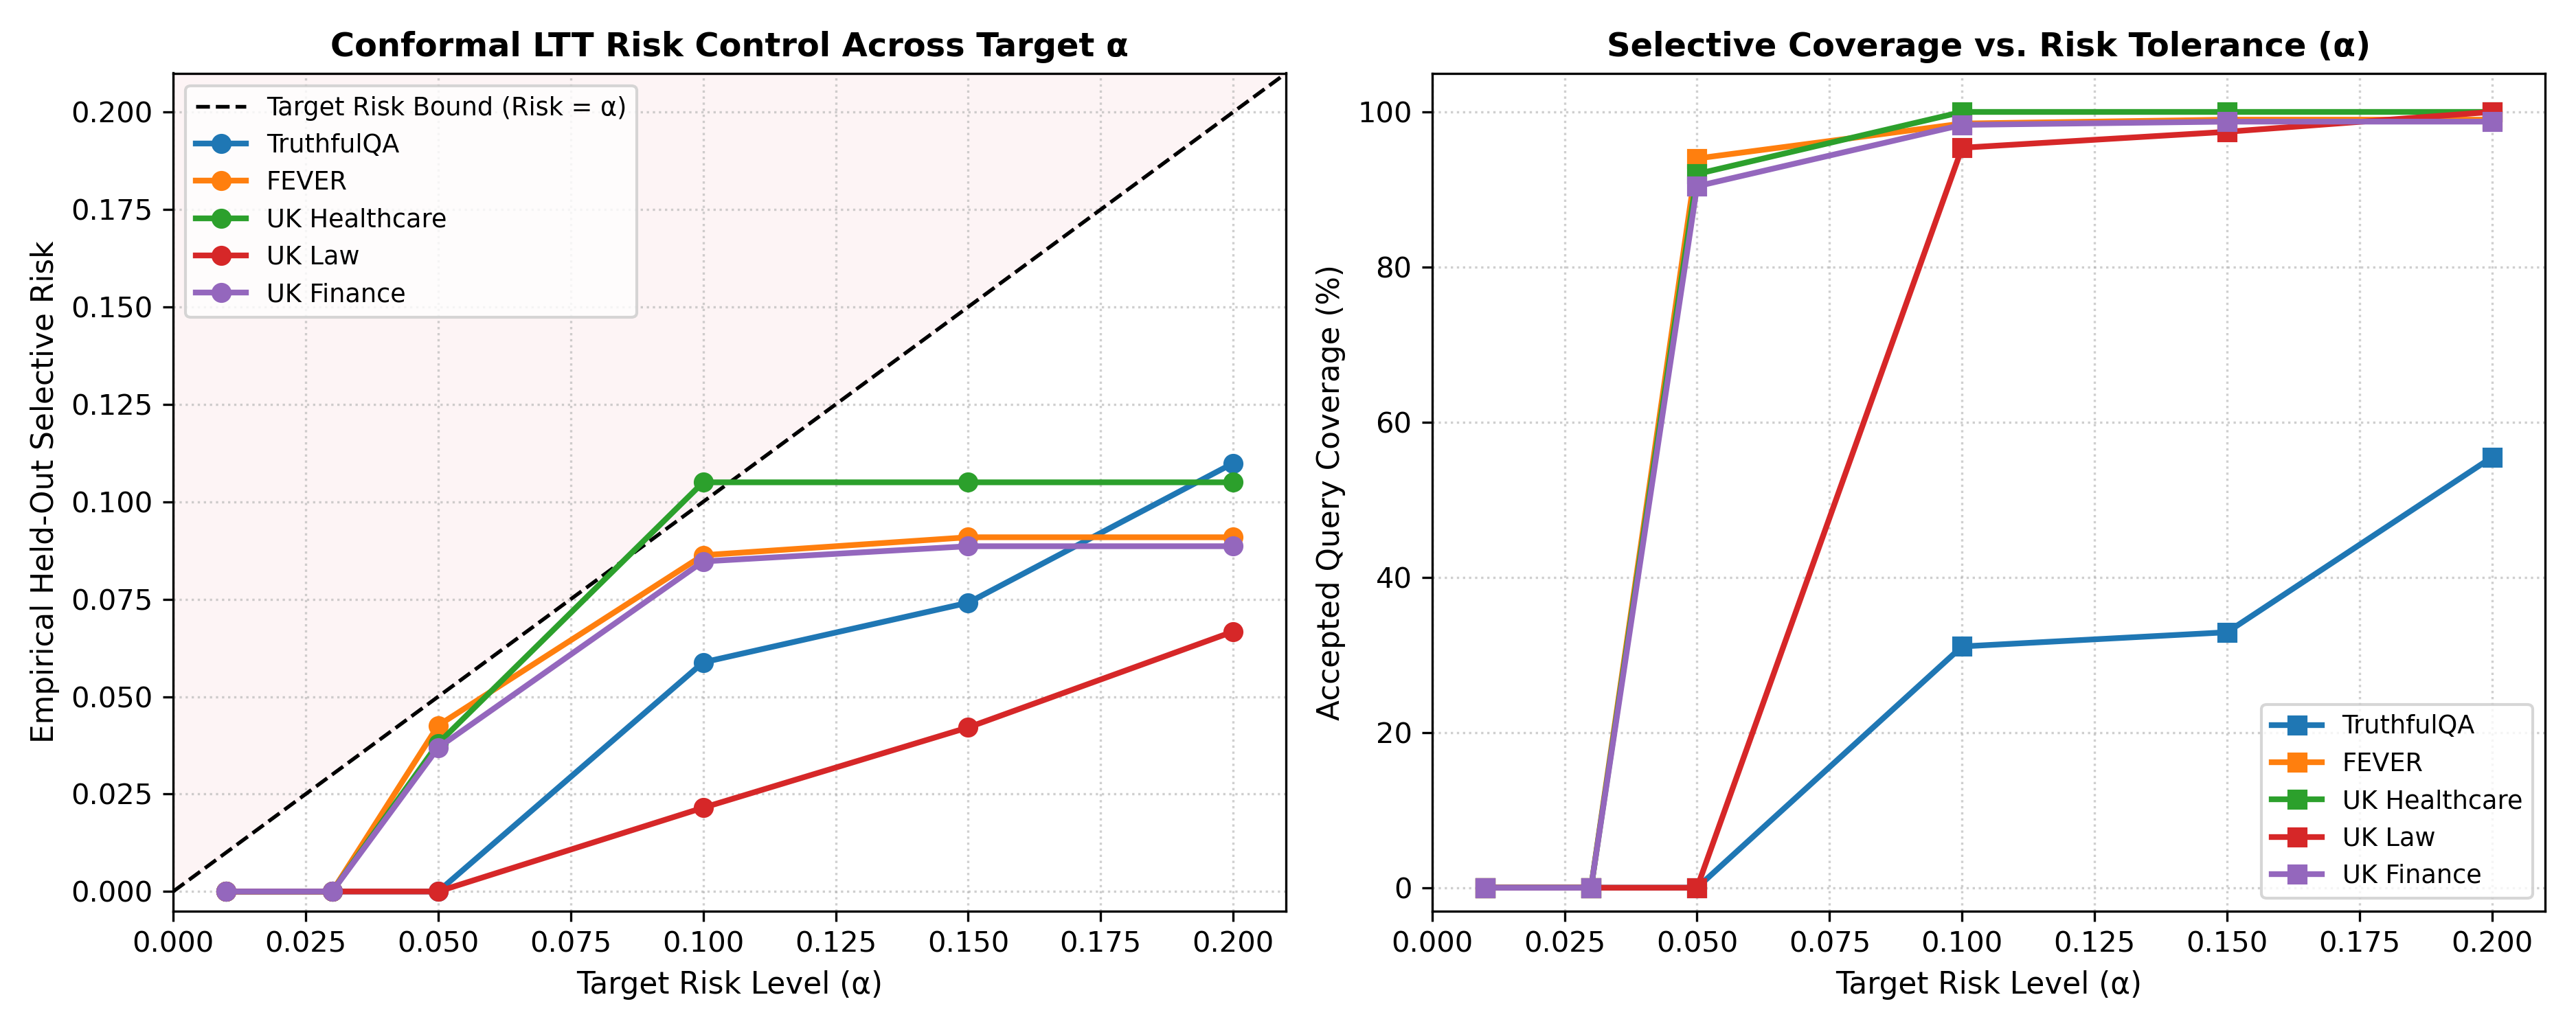
\includegraphics[width=\linewidth]{../results/figures/fig1_risk_coverage_alpha_sweep.png}
\caption{Empirical selective risk vs.\ target $\alpha$ across all five domains, demonstrating strict adherence below the $y=\alpha$ risk boundary.}
\label{fig:risk_sweep}
\end{figure}

\begin{figure}[t]
\centering
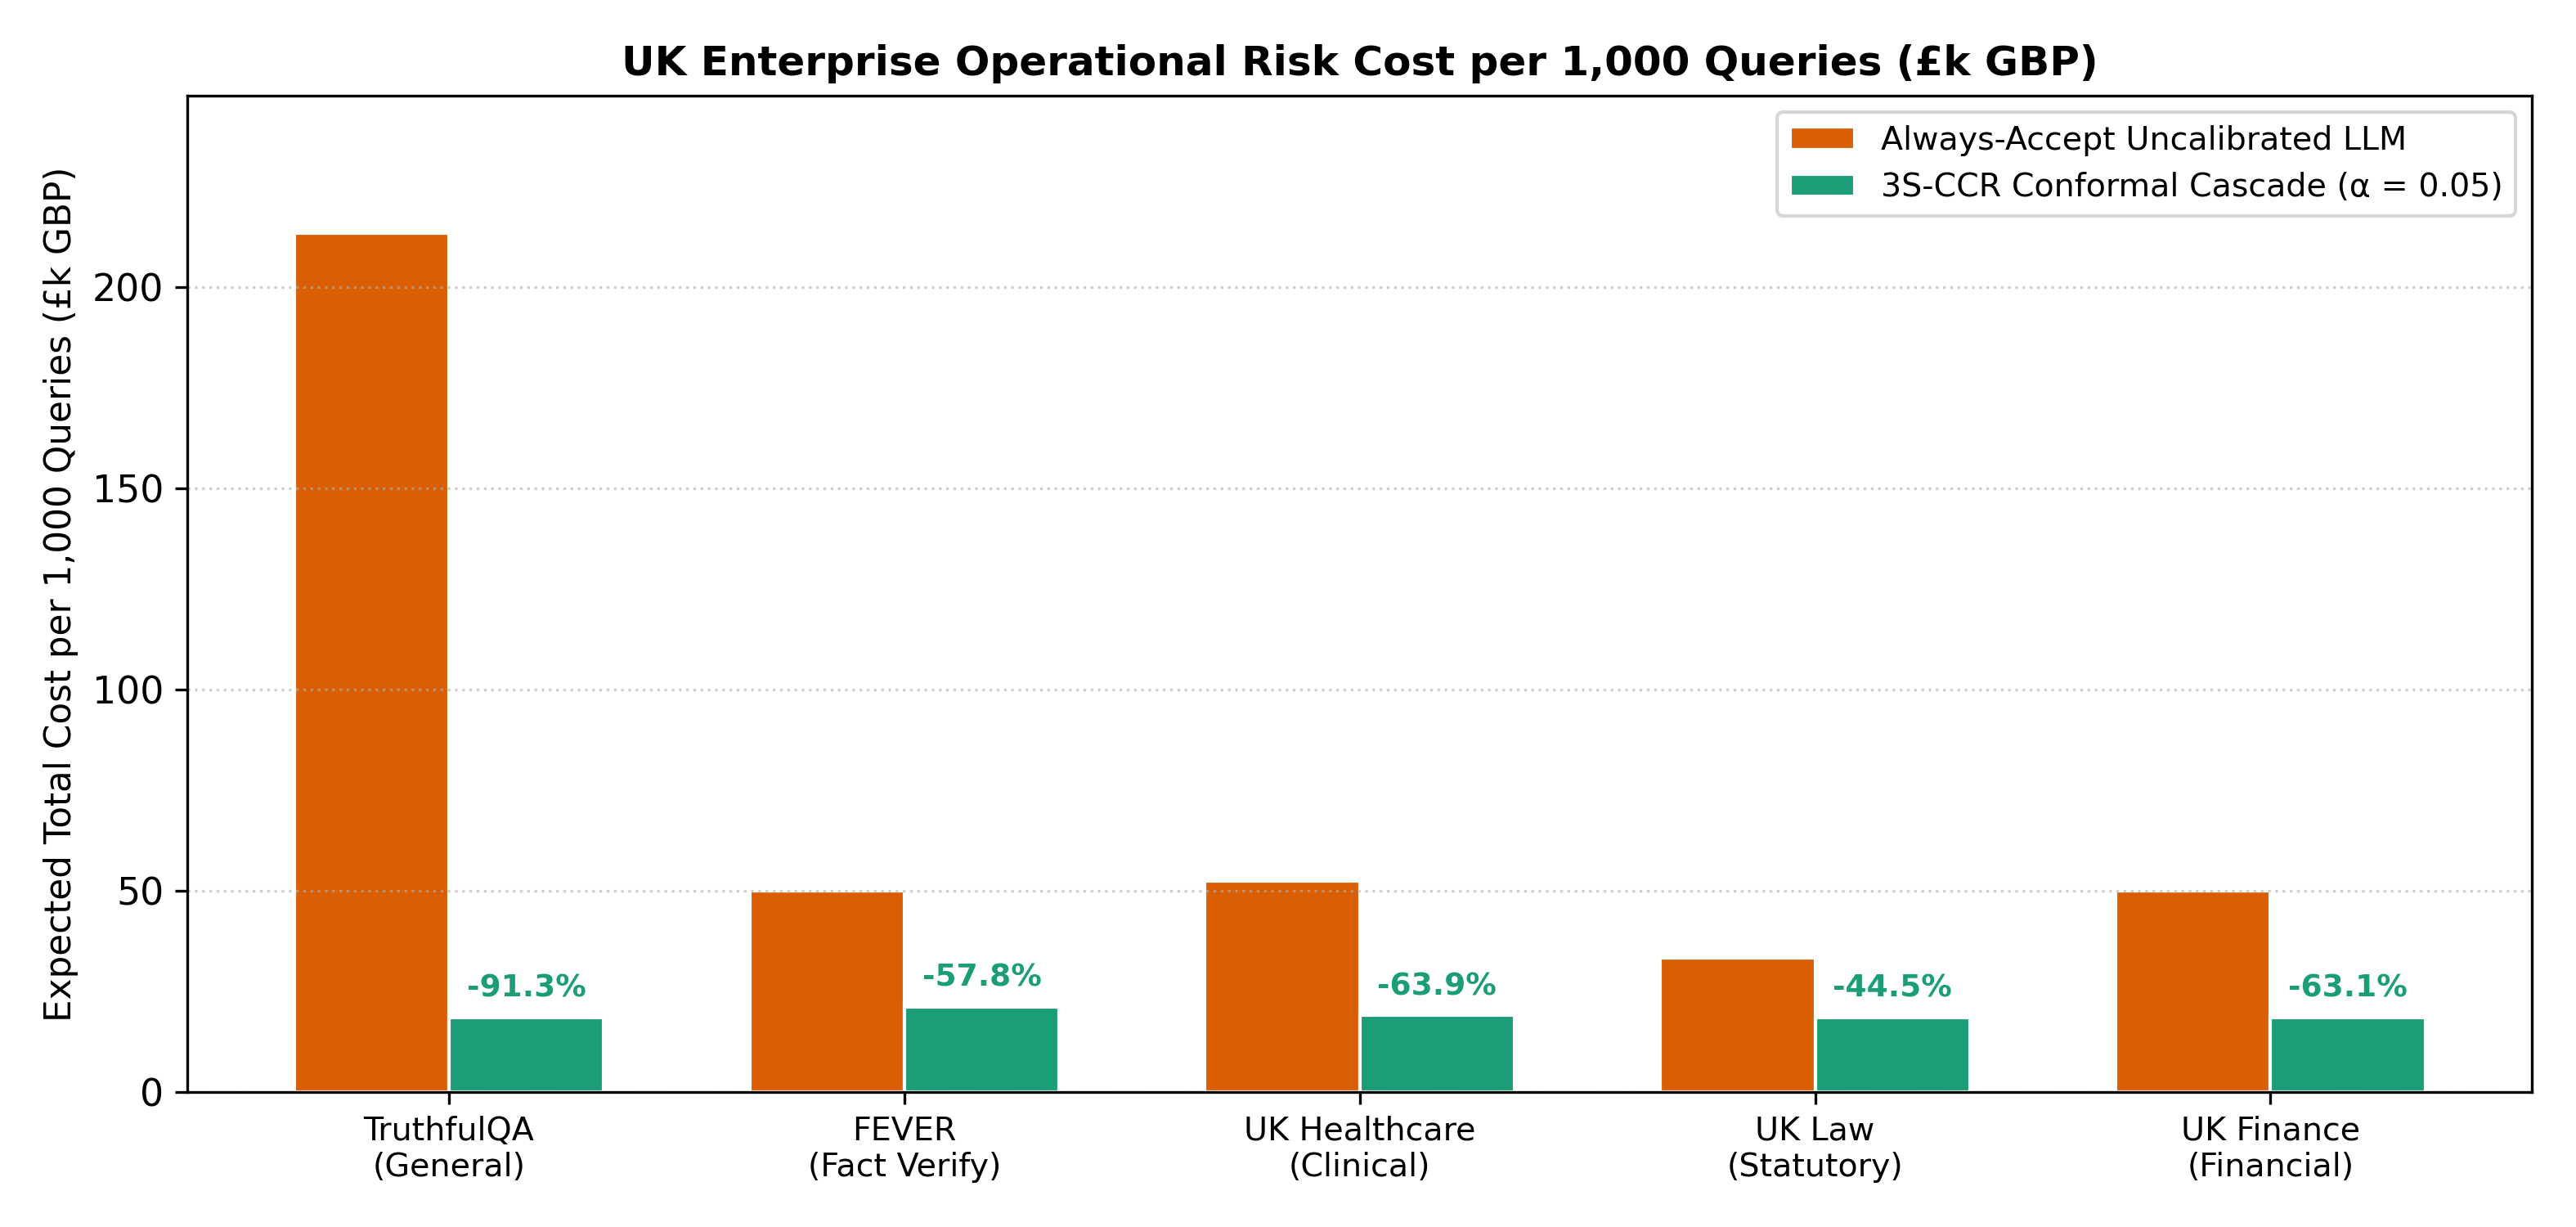
\includegraphics[width=\linewidth]{../results/figures/fig3_uk_enterprise_economics.png}
\caption{Expected operational risk cost per 1,000 queries (\pounds k GBP) comparing uncalibrated always-accept routing against 3S-CCR.}
\label{fig:economics}
\end{figure}

\section{Conclusion}
3S-CCR bridges statistical conformal prediction and cost-aware cascade routing, providing provable hallucination control and substantial operational cost savings across regulated UK enterprise domains.

\end{document}
